\chapter{Understanding Transformers}
\label{C:transformers}

Many of the recent amazing results in deep learning have been achieved with a class of neural networks called \textit{transformers}, which were introduced and named in "Attention Is All You Need", Vaswani et al. 2017 \cite{attention-is-all-you-need}. The distinguishing feature of these models is using one or more \textit{attention} layers to enable information propagation between elements in sequence data. Since 2017, a large number of transformer variants have been developed, and in this chapter I seek to understand this class of models at a broader level. I will discuss:

\begin{itemize}
    \item The unique properties of the attention operation, which include working with sequences of any length without changing the weights, being able to be computed in parallel across the sequence during training, and being invariant to the order of the inputs.
    \item The different variants of transformers, namely encoder-only, decoder-only, and encoder-decoder models.
    \item The variety of different tasks that these model are trained on and used for, building up to the next chapter where I introduce an extremely generic gaussian-process-like task.
\end{itemize}

Firstly, I will discuss the attention operation that under-pins transformers.

\section{The Attention Operation}

Attention is a biologically-inspired mechanism that allows a model to recieve inputs from distant parts of the input data, weighted by the \textit{attention weight} given to those inputs, which is typically computed from the data itself. This has proven extremely useful for diverse tasks including machine translation, image generation, and more. In this section I will describe the attention operator.

Attention has a number of useful properties which come from its mathematical construction, such as permutation-invariance in the inputs.

\subsection{Mathematical Definition}

An attention operation is of the following form, using short summation notation, where $\sigma$ is the \textit{softmax} operator (see \ref{eqn:softmax}), and $A$ is the pre-softmax attention logits.
\vspace{-10pt}
\begin{gather*}
    \nfdef{f_{\text{attn}}}{\R^{M×D}×\R^{N×D}×\R^{N×V}}{\R^{M×V}}
\end{gather*}
\vspace{-10pt}
\begin{equation}
\label{eqn:attn}
\begin{split}
    f_{\text{attn}}(Q, K, V)_{mv} ≝ \sum_n \left[\sigma\Big(\sum_d Q_{md} K_{nd}\Big) _{mn} V_{nv} \right]
\end{split}
\end{equation}%
\begin{gather*}
    Q ∈ \R^{M×D}, K ∈ \R^{N×D}, V ∈ \R^{N×V} \\
    M, N, D, V ∈ \N
\end{gather*}\vspace{-10pt}\\
The innermost multiplication of $Q$ and $K$ is simply the inner product (dot product) between vectors $Q_m$ and $K_n$. This however is not inherent. Instead of the inner product, we can substitute any kernel function. (Although this is not usually done because the inner product is the most natural choice, and is efficient to compute)

For clarity, the expanded form of the attention computation, resulting in the unnormalized attention weights $A$, for an arbitrary kernel function $k$, is as follows:
\begin{align*}
A_{mn} = k(Q_m, K_n)
&= \begin{bmatrix}
    k(Q_{1}, K_{1}) & k(Q_{1}, K_{2}) & \cdots & k(Q_{1}, K_{N}) \\
    k(Q_{2}, K_{1}) & k(Q_{2}, K_{2}) & \cdots & k(Q_{2}, K_{N}) \\
    \vdots & \vdots & \ddots & \vdots \\
    k(Q_{M}, K_{1}) & k(Q_{M}, K_{2}) & \cdots & k(Q_{M}, K_{N})
\end{bmatrix} \\
\text{or when\ } k(a, b) = a \cdot b &\text{, then} \\
&= \begin{bmatrix}
    Q_{1,1} & Q_{1,2} & \cdots & Q_D \\
    Q_{2,1} & Q_{2,2} & \cdots & Q_D \\
    \vdots & \vdots & \ddots & \vdots \\
    Q_{M,1} & Q_{M,2} & \cdots & Q_D
\end{bmatrix} \begin{bmatrix}
    K_{1,1} & K_{1,2} & \cdots & K_D \\
    K_{2,1} & K_{2,2} & \cdots & K_D \\
    \vdots & \vdots & \ddots & \vdots \\
    K_{N,1} & K_{N,2} & \cdots & K_D
\end{bmatrix}^T \\
&= Q K^T .
\end{align*}

We can see that the attention weights $A$ have shape $M×N$. This is the primary drawback of the attention operation. $M$ and $N$ are typcially both large, and the takes $O(MN)$ space and time to compute. Despite this drawback, the attention operation has proven extremely useful in a variety of tasks. There are many different ways to address this but I will not discuss them.

\subsection{Permutation-invariance with respect to $K$ and $V$}

The first interesting property of attention is that it is permutation-invariant with respect to the key and value inputs. This property is more or less useful depending on the task. For example, in the case of graphs, or sets of heterogeneous values, there may not be a natural ordering in which to process the inputs. In this case, we do not have to introduce any artificial ordering. (However, when \textit{sampling} outputs, we typically still need to decide on some order. I will discuss this in more detail in \Cref{C:a-o-sampling}).

This property is due to the construction of the attention operator. We can see that the output $O_m$ corresponding to a query vector $Q_m$ is independent of the order of the key and value vectors $K_n$ and $V_n$, because the summation across $n$ is commutative:
\begin{align}
\label{eqn:attn-perm-invariance}
\begin{aligned}
    O_m &= \sum_n V_n \sigma(A_{m})_n
\end{aligned}
\end{align}

\subsection{Permutation-equivariance with respect to $Q$}

Relatedly, attention is also permutation-\textit{equivariant} with respect to the query inputs. Equivariance means that the value of the output $O_m$ is dependent on the value of the query vector $Q_m$, but independent of the order of all other query vectors $Q_{m'}$, $m' ≠ m$.
This property is due to the fact that softmax operation is equivariant to the order of its inputs, which we can see from the construction in \Cref{eqn:softmax}.

This property of attention stands in contrast to the two main other methods used to process sequence data, convolution (CNNs) and recurrence (RNNs). Neither of these operations are invariant (or equivariant) with respect to their inputs.

\subsection{Dynamic length inputs}

The second (and most useful) property of attention is that it can be used to process inputs of dynamic length. We can again see why this is the case from \Cref{eqn:attn-perm-invariance}. The softmax operation normalizes the attention weights, which causes the resulting summation of vectors $V_n$ to be a convex combination. The resulting output $O_m$ will therefore sit within the convex hull of the vectors $V_n$. This means that the output $O_m$ will be a ``valid'' output regardless of the length of the input sequence $K_v$.

\subsection{Parallel computation}

The third property of attention is that it can be computed in parallel across the inputs sequence during training. At all steps of the attention computation except the softmax operation, there are no dependencies between neghbouring elements of the tensors. This stands in contrast to RNNs, where the outputs for one position in the sequence depend on the previous outputs.

The fact that attention can be computed in parallel is a very useful property, since while the operation requires $O(MN)$ time and space, we can utilize bigger GPU hardware the real-time cost to $O(1)$ (assuming sufficient memory capacity, compute capability, and also GPU memory bandwidth, which is often the limiting factor \cite{multi-query-attn}.) The attention logits $A_{mn}$ can be computed entirely in parallel. The softmax operation depends on all previous attention logits across the key-value dimension $N$, which requires cross-talk between GPU units but does not prevent parallel computation. The final computation for the outputs $O_m$ can also be computed in parallel.

So attention is a operation with a number of useful properties. Now we will see how it is used to build a variety of models capable of solving a variety of tasks with sequence data.

\section{Transformer models}

An attention operation model does not itself make a neural network. It is simply a building block that can be used to construct a neural network.

A transformer model puts attention operations together with MLP blocks similarly to in residual networks (ResNets). Without MLP blocks as non-linearities, the outputs of an attention operation are linear functions of the inputs, since the softmax is only used to compute coefficients when summing the values. This means that the outputs of an attention operation are linear combinations of the inputs. This is useful as a building block but we would like to be able to learn non-linear functions of the inputs. MLP blocks are used to introduce non-linearities into the model.

In \Cref{fig:residual-block} we can see a diagram of a typical residual block in a transformer, combining an attention operation, a feed-forward layer, and a residual connection as in a ResNet.

\begin{figure}
    \centering
    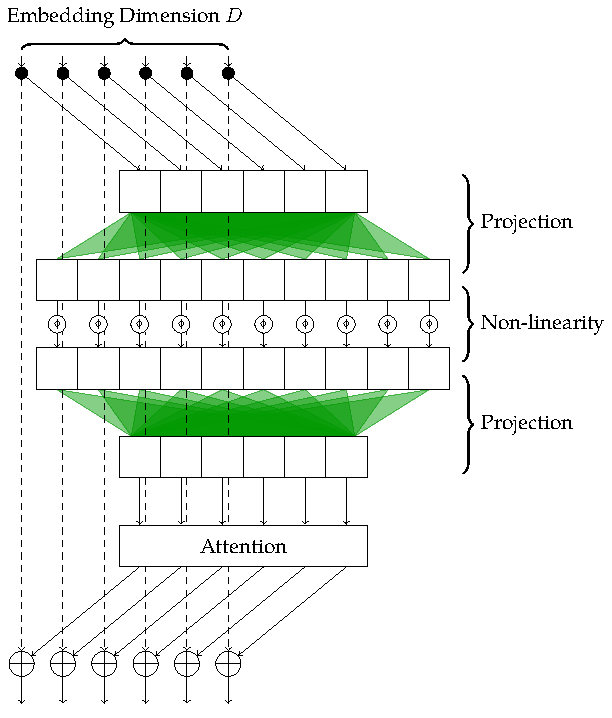
\includegraphics[]{figures/residual-block.pdf}
    \captionsetup{parskip=7pt}
    \caption[Typical residual block in transformer]{Typical residual block in transformer (with the $D$ dimension expanded, rather than the $N$ or $M$ dimension as usual.).

    In the MLP block, the sequence of residual latents are independently projected into a higher-dimensional space, where a non-linearity is applied, and then projected back down to the original dimension. The output of the MLP block is then projected into $Q$, $K$, and $V$ spaces, and the attention operation is applied. Finally, the results are added to the residual stream.}
    \label{fig:residual-block}
\end{figure}

Attention is computed from the three matrices (or sequences of vectors) $Q$, $K$ and $V$. In a neural network, these are each typically derived in some fashion from the inputs to the network. The most common way to do this is to use a learned linear transformation, which is simply a matrix multiplication followed by a bias term, for example
\begin{align}
\begin{aligned}
\label{eqn:attn-linear}
Q &= W_{Q} \X + \vb_{Q} \\
K &= W_{K} \X + \vb_{K} \\
V &= W_{V} \X + \vb_{V}
\end{aligned}
\end{align}
If we derive all three matrices from the same input $\X$, then $M = N$ and the attention operation is called a \textit{self-attention} operation. A diagram of this is shown in \Cref{fig:self-attn}. The blue shaded areas show the receptive field used when computing each output vector $x'_i$.

When Q and K are derived from separate sequences of feature/embedding vectors, then in general $M ≠ N$ and this is called \textit{cross-attention}. A diagram of this is shown in \Cref{fig:cross-attention}.

\begin{figure}
    \centering
    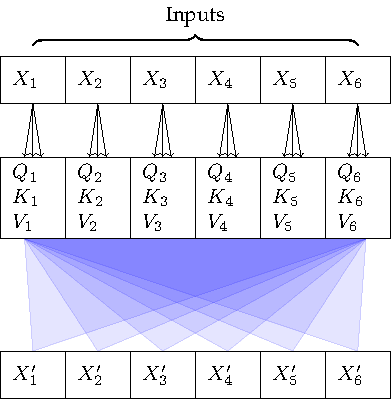
\includegraphics[]{figures/attn-1-self.pdf}
    \caption[Self-attention]{Full self-attention (bi-directional attention), as used in transformer encoders. The blue shaded regions show which inputs are used to compute each output. In full self-attention, all inputs are used to compute all outputs.}
    \label{fig:self-attn}
\end{figure}


\begin{figure}
    \centering
    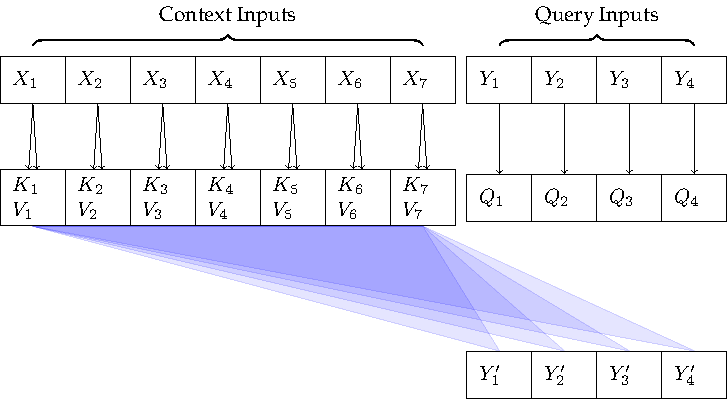
\includegraphics[]{figures/attn-2-cross.pdf}
    \caption[Cross-attention]{Cross-attention, as used in encoder-decoder models.}
    \label{fig:cross-attn}
\end{figure}

Since the introduction of transformers it is common to use \textit{multi-head} attention, which allows for multiple \textit{heads} which each perform an attention operation in parallel with smaller key dimensionality $D_{\text{head}} = \frac{D}{ n_{\text{heads}}}$.

The defining feature of a transformer model is that it has ``attention'' layers. However, there is not just one way to assemble these layers, and there is not just one way to train these models.

We can broadly split the transformer architecture variants into four categories: \textit{encoder-only} models, \textit{decoder-only} models, unified attention models, and \textit{encoder-decoder} models.

\subsection{Masked Sequence Modeling: Encoder-only models}
\label{ss:msm}

Arguably the simplest attention-based model architecture is encoder-only transformers. When used in natural-language-processing (NLP) they are known as bi-directional language models, because they allow information to flow in both directions. Examples are the BERT \cite{bert} language model family, Wav2Vec \cite{wav2vec} for speech, and SimMIM \cite{sim-mim} image model.

These models are trained on a sequence reconstruction task, called Masked Language Modeling (MLM), Masked Image Modeling (MIM), or more generally Masked Sequence Modeling, which I will discuss more in \Cref{ss:pretraining}.

These models are typically used for sequence understanding tasks and classification tasks, however they can also be used for generating sequences. The limitation of these kinds of models is that their pretraining task is not efficient for training these models to generate sequences. For generating sequences, an encoder model in conjunction with a \textit{decoder} model (see \Cref{ss:encoder-decoder}), or simply a decoder-only model.

\subsection{Sequence Prediction: Decoder-only models}
\label{ss:decoder-only}

A diagram of the decoder-only architecture, is shown below in \Cref{fig:decoder-only}. The distinguishing feature of a \textit{decoder} as opposed to an encoder is that its attention layers are all causally-masked self-attention layers as in \Cref{fig:self-attn-causal}. These models are used for sequence prediction/generation, and trained via self-supervised learning.

Some examples of where we see this architecture in use are:
\begin{itemize}
    \item OpenAI's GPT-series \cite{gpt2, gpt3} language models.
    \item Latent code prediction (the ``prior'') in VQ-GAN \cite{vqgan}
\end{itemize}


\begin{figure}
    \centering
    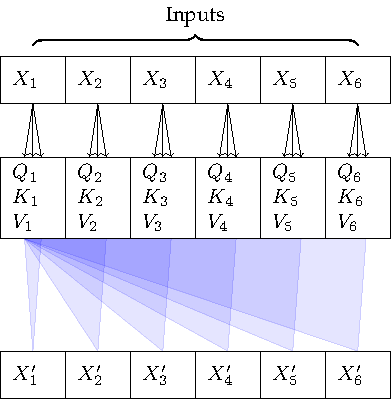
\includegraphics[]{figures/attn-3-causal.pdf}
    \caption[Self-attention with causal masking]{Self-attention with causal masking, (uni-directional attention) as used in transformer decoders during training. The blue shaded regions show which inputs are used to compute each output. In causal masking, only inputs to the left of the current output are used to compute the current output.}
    \label{fig:self-attn-causal}
\end{figure}

\begin{figure}
    \centering
    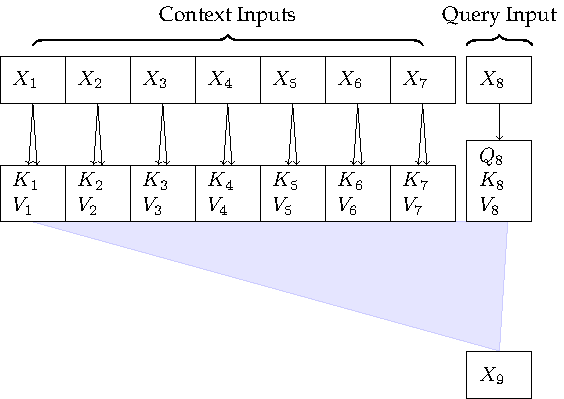
\includegraphics[]{figures/attn-4-partial.pdf}
    \caption[Partial self-attention]{Partial self-attention, as used during incremental autoregressive inference (in models with a decoder).}
    \label{fig:partial-self-attn}
\end{figure}


\begin{figure}
    \centering
    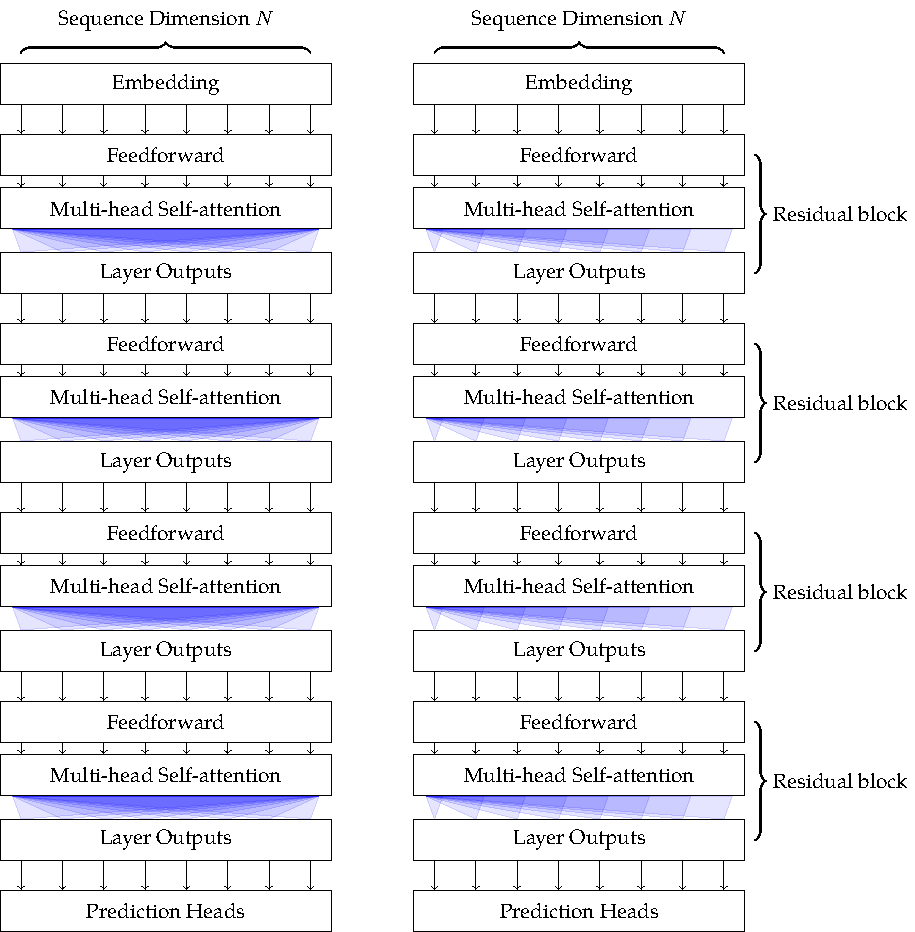
\includegraphics[width=1.2\linewidth]{figures/transformers.pdf}
    \caption[Transformer model]{Left: Encoder-only model. Right: Deocder-only model. Residual connections have been ommitted for brevity.}
    \label{fig:transformers}
\end{figure}


\subsection{Encoder-decoder models}
\label[]{ss:encoder-decoder}

When the transformer was introduced in \cite{attention-is-all-you-need}, the first architecture proposed was an encoder-decoder architecture. This is a model which has both an encoder and a decoder. The encoder is used to encode a sequence of \textit{conditioning} or \textit{context} inputs, and the decoder is used to generate the output sequence. The encoder and decoder are connected by cross-attention layers (see \Cref{fig:cross-attn}), which allow the decoder to attend to the encoded context sequence.

These are the most flexible class of model, because they allow predicting some outputs, or sequences of outputs, \textit{given} some inputs.

Examples of this are the original transformer architecture \cite{attention-is-all-you-need}, the BART \cite{bart} model, and more recently Google's Parti multi-modal text-to-image model \cite{parti}.

In \cite{attention-is-all-you-need}, they train an encoder-decoder architecture for text translation. Their architecture takes one sequence of text tokens (if you are wondering what text tokens are, I will discuss input formats in the next section) in language A as conditioning input, then auto-regressively samples a target sequence in a second language B. The two languages may have very different word orderings or numbers of words to each other, but the cross-attention operation introduces no bias towards aligned word orderings or even word counts.

\subsection{Unified attention models}

\begin{figure}
    \centering
    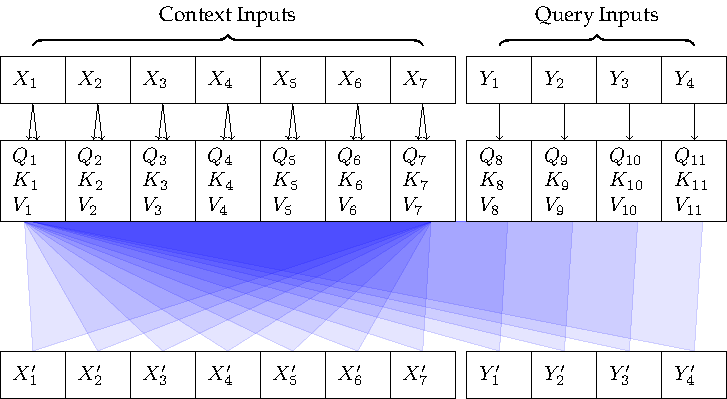
\includegraphics[]{figures/attn-5-unified.pdf}
    \captionsetup{parskip=7pt}
    \caption[Unified attention]{Unified self- and cross-attention, as in \cite{unilm}.

    Bi- and uni-directional attention can be performed with the same attention layers with careful masking, allowing the same model to be trained on any mixture of pre-training tasks.

    The ``encoder'' outputs $X'$ are computed with full self-attention, and the ``decoder'' outputs $Y'$ are computed with full attention with respect to $X$ and causal attention with respect to $Y$.}
    \label{fig:unified-attn}
\end{figure}

As we see in \ref{fig:unified-attn}, there are actually two ways we might include information from the encoded sequence into the decoded sequence. In the first, which is used in most encoder/decoder models including the original, all the layers of the encoder are computed fully, and the final encoded sequence is provided to the decoder at all layers via cross-attention. In the second, the encoder is separated from the decoder only by correct application of masking in the attention layers, and is only computed up to the layer which is being decoded at.

\begin{figure}
    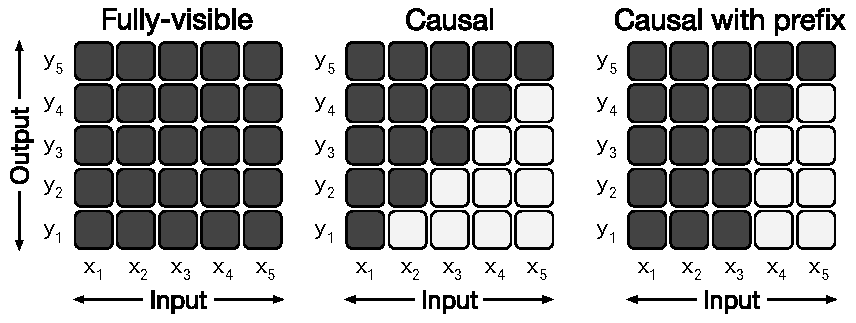
\includegraphics[width=\linewidth]{figures/attention_masks.pdf}
    \caption[Attention Masks]{Masking in unified attention layers \cite{unilm,t5}. The bi- and uni-directional attention can be performed within a single attention layer.}
    \label{fig:unified-masking}
\end{figure}

The different layouts that can be used are shown in \Cref{fig:unified-masking}.

The first method is more efficient because the attention matrices of the encoder and the decoder are split, using $O(N^2 +M^2)$ memory rather than $O(N^2M^2)$. However, the second method is conceptually simpler and is better when the trained model will be used for fine-tuning/transfer learning \cite{t5}., because it uses the  decoder to attend to the encoded sequence at any layer, and not just the final layer. This is useful for tasks such as image captioning, where the decoder may want to attend to the encoded image at multiple layers, and not just the final layer.

Tranformer models trained on a mix of pre-training tasks using this architecture are known as T5 models (\textbf{T}ext-\textbf{T}o-\textbf{T}ext \textbf{T}ransfer \textbf{T}ransformers) \cite{t5}.


\section{Pretraining tasks}
\label{s:pretraining}

A \textit{pre-training task} is a self-supervised task used to train a transformer. There are two main pre-training methods for transformer models which I have already mentioned: \textit{Masked Sequence Modeling} and \textit{Auto-regressive Sequence Modeling} (ASM).

In masked sequence modeling (MSM), the model is trained to reconstruct the original sequence, but with some of the inputs masked out. An example of this for a language model is shown in \Cref{fig:xlm}.

\begin{figure}
    \centering
    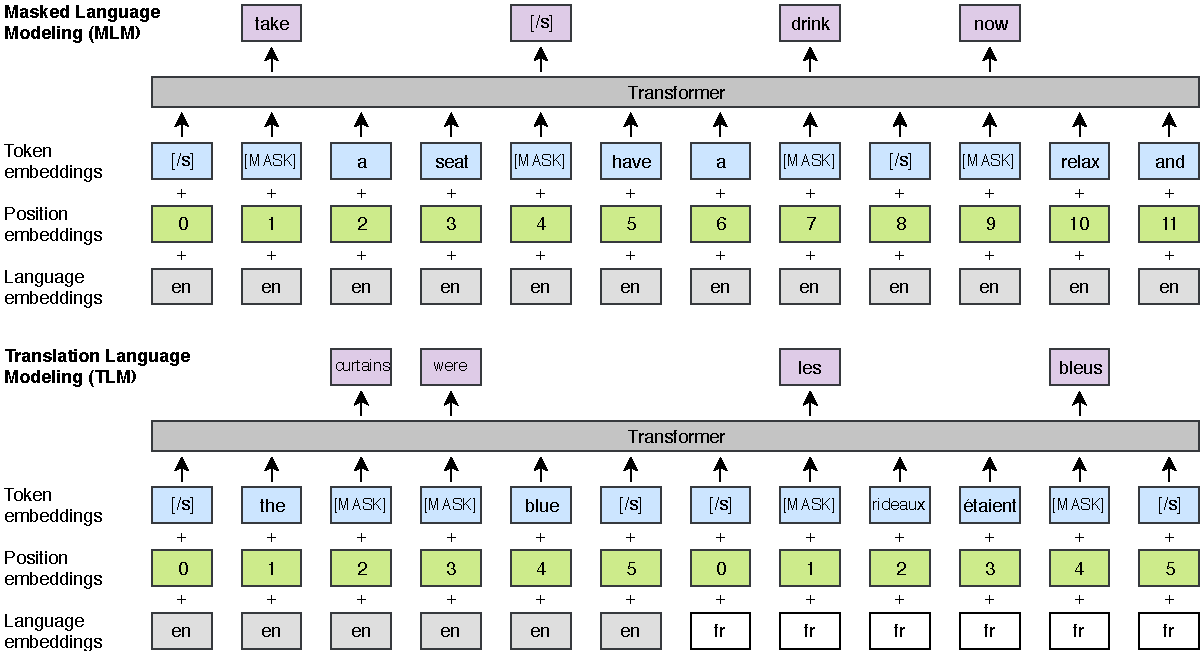
\includegraphics[width=\linewidth]{figures/XLM.pdf}
    % \vspace{-0.4cm}
    \caption[Masked Language Model Pretraining]{Cross-lingual masked language model pretraining, from \cite{cross-lingual-mlm}.

    Top: The standard MLM pretraining task. A sequence of text tokens are given as input, some are masked and the model is trained to predict the masked tokens.

    Bottom: The cross-lingual MLM pretraining task. A sequence of text tokens from two different languages are given as input, some tokens are masked and the model is trained to predict the masked tokens. The model is trained on a mixture of monolingual and cross-lingual examples.}
    \label{fig:xlm}
\end{figure}

\begin{figure}
    \centering
    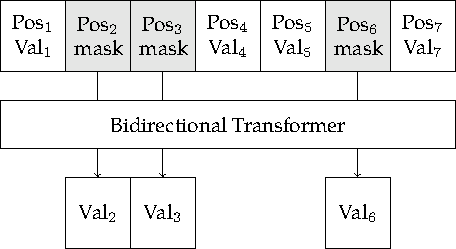
\includegraphics[width=\linewidth]{figures/pretraining-msm.pdf}
    \caption[Masked Sequence Modeling Pretraining]{Masked sequence modeling pretraining task. The model is trained to reconstruct masked-out elements of the original sequence.}
    \label{fig:pretraining-msm}
\end{figure}

\begin{figure}
    \centering
    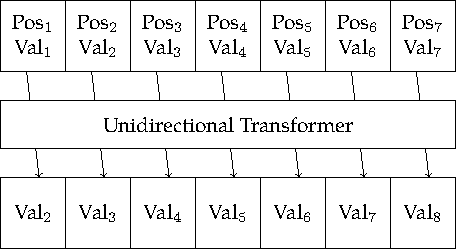
\includegraphics[width=\linewidth]{figures/pretraining-causal.pdf}
    \caption[Autoregressive Sequence Modeling Pretraining]{Autoregressive pretraining task. The model is trained to predict the next element in the sequence.}
    \label{fig:pretraining-causal}
\end{figure}

The inputs to the tranformer models are typically sequences of discrete tokens, which each have a corresponding entry in a learned codebook of latent vectors. Masking out an input in this context means adding an additional token and learned embedding``<mask>'' to the codebook, which is used to represent the masked out inputs. As we can see in the figure, the masked positions still have embeddings of the positional information, which is necessary because a transformer model has no implicit order information available to it.

The second main pre-training task is auto-regressive sequence modeling, where the model is trained to predict the next token in a sequence, given the previous tokens. For this pre-training task the target outputs are present in the input sequence, but one token ahead. The model must therefore be a uni-directional / causally-masked model (\Cref{fig:transformers}) to prevent information flow from the future to the past and prevent the model learning degenerate behaviour., as in \Cref{fig:self-attn-causal}.


% attention
% transformer architectures
% pre-training types

In the next chapter (\Cref{C:a-o-sampling}) I experiment with a new pre-training task, which is a variation on auto-regressive sequence modeling, which I call \textit{arbitrary-order autoregressive pretraining}, which I will later apply to hand motion prediction.
